\documentclass[14pt]{beamer}
\usepackage{./Estilos/BeamerUVM}
\usepackage{./Estilos/ColoresLatex}
\usetheme{Madrid}
\usecolortheme{default}
%\useoutertheme{default}
\setbeamercovered{invisible}
% or whatever (possibly just delete it)
\setbeamertemplate{section in toc}[sections numbered]
\setbeamertemplate{subsection in toc}[subsections numbered]
\setbeamertemplate{subsection in toc}{\leavevmode\leftskip=3.2em\rlap{\hskip-2em\inserttocsectionnumber.\inserttocsubsectionnumber}\inserttocsubsection\par}
% \setbeamercolor{section in toc}{fg=blue}
% \setbeamercolor{subsection in toc}{fg=blue}
% \setbeamercolor{frametitle}{fg=blue}
\setbeamertemplate{caption}[numbered]

\setbeamertemplate{footline}
\beamertemplatenavigationsymbolsempty
\setbeamertemplate{headline}{}


\makeatletter
% \setbeamercolor{section in foot}{bg=gray!30, fg=black!90!orange}
% \setbeamercolor{subsection in foot}{bg=blue!30}
% \setbeamercolor{date in foot}{bg=black}
\setbeamertemplate{footline}
{
  \leavevmode%
  \hbox{%
  \begin{beamercolorbox}[wd=.333333\paperwidth,ht=2.25ex,dp=1ex,center]{section in foot}%
    \usebeamerfont{section in foot} {\insertsection}
  \end{beamercolorbox}%
  \begin{beamercolorbox}[wd=.333333\paperwidth,ht=2.25ex,dp=1ex,center]{subsection in foot}%
    \usebeamerfont{subsection in foot}  \insertsubsection
  \end{beamercolorbox}%
  \begin{beamercolorbox}[wd=.333333\paperwidth,ht=2.25ex,dp=1ex,right]{date in head/foot}%
    \usebeamerfont{date in head/foot} \insertshortdate{} \hspace*{2em}
    \insertframenumber{} / \inserttotalframenumber \hspace*{2ex} 
  \end{beamercolorbox}}%
  \vskip0pt%
}
\makeatother

\makeatletter
\patchcmd{\beamer@sectionintoc}{\vskip1.5em}{\vskip0.8em}{}{}
\makeatother

% \usefonttheme{serif}
\usepackage[clock]{ifsym}

\sisetup{per-mode=symbol}
\DeclareSIUnit{\dB}{dB}
\resetcounteronoverlays{saveenumi}

\title{\Large{Hidrodinámica} \\ \normalsize{Física IV (área II)}}
\date{}

% Macro para agregar el logo de UVM en cada slide de la presentación

\addtobeamertemplate{frametitle}{}{%
\begin{tikzpicture}[remember picture,overlay]
\coordinate (logo) at ([xshift=-1.5cm,yshift=-0.8cm]current page.north east);
% \fill[devryblue] (logo) circle (.9cm);
% \clip (logo) circle (.75cm);
\node at (logo) {
\includegraphics[width=2.1cm]{Imagenes/logo_UVM.png}};
\end{tikzpicture}}


\begin{document}
\maketitle

\section*{Contenido}
\frame[allowframebreaks]{\frametitle{Contenido} \tableofcontents[currentsection, hideallsubsections]}

\section{Hidrodinámica}
\frame{\tableofcontents[currentsection, hideothersubsections]}
\subsection{Definición}

\begin{frame}
\frametitle{¿Qué es la hidrodinámica}
La \textocolor{ao}{hidrodinámica} es la parte de la \textocolor{cadmiumgreen}{mecánica de fluidos} cuyo propósito es el estudio de los \textocolor{lava}{fluidos en movimiento}.
\\
\bigskip
\pause
En sentido restringido, estudia el comportamiento del agua en movimiento.
\end{frame}
\begin{frame}
\frametitle{Tipos de fluidos}
Para facilitar la comprensión del estudio de los fluidos en movimiento debemos considerar que los fluidos son ideales, es decir, que poseen las siguientes características:
\end{frame}
\begin{frame}
\frametitle{Tipos de fluidos}
\setbeamercolor{item projected}{bg=bananayellow,fg=ao}
\setbeamertemplate{enumerate items}{%
\usebeamercolor[bg]{item projected}%
\raisebox{1.5pt}{\colorbox{bg}{\color{fg}\footnotesize\insertenumlabel}}%
}
\begin{enumerate}[<+->]
\item \textocolor{byzantium}{Incompresible.} La densidad es constante y uniforme.
\item \textocolor{cobalt}{Flujo constante.} La velocidad no cambia con el tiempo, aunque puede ser diferente en distintos puntos.
\seti 
\end{enumerate}
\end{frame}
\begin{frame}
\frametitle{Tipos de fluidos}
\setbeamercolor{item projected}{bg=bananayellow,fg=ao}
\setbeamertemplate{enumerate items}{%
\usebeamercolor[bg]{item projected}%
\raisebox{1.5pt}{\colorbox{bg}{\color{fg}\footnotesize\insertenumlabel}}%
}
\begin{enumerate}[<+->]
\conti
\item \textocolor{carmine}{No viscoso.} Sin fricción. Las fuerzas son conservativas.
\item \textocolor{bulgarianrose}{Irrotacional.} Las partículas sólo tienen movimiento de traslación.
\end{enumerate}
\end{frame}
\begin{frame}
\frametitle{El gasto}
El \textocolor{cornellred}{gasto o caudal} es el volumen de fluido que pasa por unidad de tiempo en una sección de conducto.
\end{frame}
\begin{frame}
\frametitle{El gasto}
\begin{figure}
    \centering
    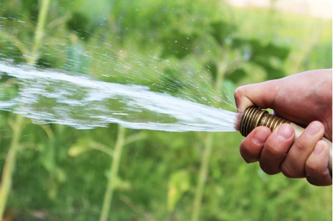
\includegraphics[scale=1]{Imagenes/Gasto_01.png}
\end{figure}
\end{frame}
\begin{frame}
\frametitle{Expresión para el gasto}
El gasto $G$ se expresa de la siguiente manera:
\pause
\begin{align*}
G = \dfrac{V}{t} \hspace{0.75cm} \Rightarrow \hspace{0.75cm} \left[ \si[per-mode=fraction]{\cubic\meter\per\second} \right]
\end{align*}
\end{frame}
\begin{frame}
\frametitle{Definición alterna al gasto}
El gasto también se puede calcular si conocemos la velocidad que lleva el fluido y la sección transversal de la tubería.
\begin{figure}
    \centering
    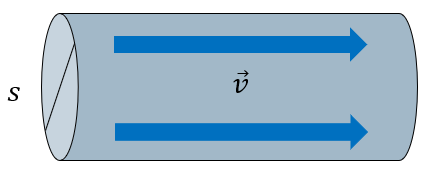
\includegraphics[scale=0.65]{Imagenes/Gasto_02.png}
\end{figure}
\end{frame}
\begin{frame}
\frametitle{Definición alterna al gasto}
El volumen se puede expresar como función del área y de la \enquote{altura}:
\pause
\begin{align*}
V = A \, h
\end{align*}
\end{frame}
\begin{frame}
\frametitle{Expresión alterna al gasto}
Entonces la expresión para el gasto resulta:
\pause
\begin{align*}
G = \dfrac{A \, h}{t}
\end{align*}
\end{frame}
\begin{frame}
\frametitle{Ajustando la expresión}
Considerando que la altura se puede expresar como una distancia \pause y sustituyendo el volumen en función del área $(A)$ y la distancia $(d)$, se obtiene lo siguiente:
\begin{eqnarray*}
\begin{aligned}
v &= \dfrac{d}{t} \\ \pause 
G &= \dfrac{A \, d}{t} = \pause A \, v
\end{aligned}
\end{eqnarray*}
\end{frame}
\begin{frame}
\frametitle{El flujo}
El flujo es la \textocolor{darkblue}{cantidad de fluido} que atraviesa una sección transversal de un ducto en una \textocolor{darkmagenta}{unidad de tiempo} y se expresa como:
\pause
\begin{align*}
\text{Flujo} = \dfrac{m}{t}
\end{align*}
\end{frame}
\begin{frame}
\frametitle{Recordando una expresión}
Si expresamos la masa $(m)$ como función de la densidad $(\rho)$, se tiene que:
\pause
\begin{align*}
m = \rho \, V
\end{align*}
\end{frame}
\begin{frame}
\frametitle{Flujo y densidad}
El flujo en términos de la densidad del líquido es:
\pause
\begin{align*}
\text{Flujo} = \dfrac{\rho \, V}{t}
\end{align*}
\end{frame}
\begin{frame}
\frametitle{Relación entre gasto y flujo}
Es posible determinar la relación entre el flujo y el gasto, ya que como mencionamos anteriormente, el gasto es:
\pause
\begin{align*}
G = \dfrac{V}{t}
\end{align*}
\end{frame}
\begin{frame}
\frametitle{Relación entre gasto y flujo}
El flujo y el gasto se relacionan por:
\pause
\begin{align*}
\text{Flujo} = G \, \rho
\end{align*}
\end{frame}

\section{Ecuación de continuidad}
\frame{\tableofcontents[currentsection, hideothersubsections]}
\subsection{Construyendo la ecuación}

\begin{frame}
\frametitle{Fluido en movimiento}
\vspace*{-0.5cm}
Cuando pasa agua o cualquier otro fluido por una tubería como la que se muestra en la figura, donde los diámetros son diferentes.
\begin{figure}
    \centering
    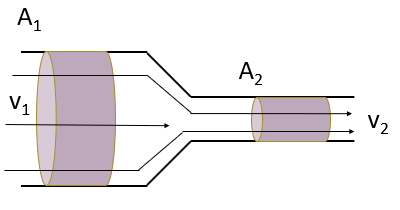
\includegraphics[scale=0.65]{Imagenes/Continuidad_01.png}
\end{figure}
\end{frame}
\begin{frame}
\frametitle{Fluido en movimiento}
\vspace*{-0.75cm}
\begin{figure}
    \centering
    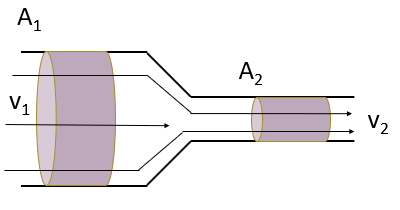
\includegraphics[scale=0.65]{Imagenes/Continuidad_01.png}
\end{figure}
El volumen del fluido \textocolor{red}{que entra} por un extremo debe \textocolor{blue}{ser igual} al volumen del fluido \textocolor{carnelian}{que sale} por el otro extremo.
\end{frame}
\begin{frame}
\frametitle{Implicación importante}
Significa que el gasto de entrada es igual al de salida, es decir:
\pause
\begin{align*}
V_{\text{entrada}} = V_{\text{salida}}
\end{align*}
\end{frame}
\begin{frame}
\frametitle{Ecuación de continuidad}
Si se conocen las \textocolor{darkscarlet}{velocidades de entrada y de salida} del fluido, \pause así como las \textocolor{debianred}{áreas de las secciones transversales} del tubo,
\end{frame}
\begin{frame}
\frametitle{Ecuación de continuidad}
Y considerando que el tiempo en que se midió el volumen de entrada es el mismo que el del volumen de salida, \pause entonces la ecuación anterior se convierte en:
\pause
\begin{align*}
v_{1} \, A_{1} = v_{2} \, A_{2}
\end{align*}
\end{frame}
\begin{frame}
\frametitle{Enunciado de un ejercicio}
Cuando el agua fluye por una manguera de \SI{0.05}{\square\meter} de área lo hace con una rapidez de \SI{1.5}{\meter\per\second}
\\
\bigskip
\pause
¿Cuál debe ser el área de la boquilla de la manguera para que salga con una rapidez de \SI{0.8}{\meter\per\second}?
\end{frame}
\begin{frame}
\frametitle{Solución al ejercicio}
\textocolor{red}{Datos:}
\pause
\begin{eqnarray*}
\begin{aligned}
A_{1} &= \SI{0.5}{\square\meter} \\ \pause
A_{2} &= \, ? \\ \pause
v_{1} &= \SI{1.5}{\meter\per\second} \\ \pause
v_{2} &= \SI{0.8}{\meter\per\second}  
\end{aligned}
\end{eqnarray*}
\end{frame}
\begin{frame}
\frametitle{Solución al ejercicio}
\textocolor{red}{Expresión:}
\pause
\begin{eqnarray*}
\begin{aligned}
v_{1} \, A_{1} = v_{2} \, A_{2} \\[0.5em] \pause
A_{2} = \dfrac{v_{1} \, A_{1}}{v_{2}}
\end{aligned}
\end{eqnarray*}
\end{frame}
\begin{frame}
\frametitle{Solución al ejercicio}
\textocolor{red}{Sustitución:}
\pause
\begin{eqnarray*}
\begin{aligned}
A_{2} &= \dfrac{\left( \SI{1.5}{\meter\per\second} \right) \left( \SI{0.5}{\square\meter} \right)}{\SI{0.8}{\meter\per\second}} = \\[0.5em] \pause
A_{2} &= \dfrac{\SI{0.75}{\cubic\meter\per\second}}{\SI{0.8}{\meter\per\second}} = \\[0.5em] \pause
A_{2} &= \SI{0.9375}{\square\meter}
\end{aligned}
\end{eqnarray*}    
\end{frame}

\section{Teorema de Bernoulli}
\frame{\tableofcontents[currentsection, hideothersubsections]}
\subsection{Observando los fluidos}

\begin{frame}
\frametitle{La ecuación de Bernoulli}
Daniel Bernoulli estudió el comportamiento de los líquidos con relación a la velocidad del fluido y la presión; descubrió que la presión de un líquido que fluye por una tubería, \textocolor{blue}{es baja} si su \textocolor{blue-violet}{velocidad es alta}.
\end{frame}
\begin{frame}
\frametitle{La ecuación de Bernoulli}
Por el contrario, \textocolor{burntorange}{la presión es alta} si su \textocolor{bole}{velocidad es baja}, \pause a esta relación se le conoce como \textocolor{cadmiumgreen}{principio de Bernoulli}.
\\
\bigskip
\pause
Además, consideró que en una tubería a mayor elevación, se tiene una menor presión.
\end{frame}

\subsection{Relación con la energía}

\begin{frame}
\frametitle{La relación con la energía}
Aplicando la conservación de la energía, Bernoulli estableció que en un flujo en el que no se agrega ni se extrae energía.
\end{frame}
\begin{frame}
\frametitle{La relación con la energía}
La energía total es constante e igual a la suma de la \textocolor{carmine}{energía cinética} (relacionado con la velocidad), \pause más la \textocolor{ao}{energía potencial} (representada por la presión) \pause más la \textocolor{coquelicot}{energía gravitacional} (relacionada con la altura).
\end{frame}

\subsection{El principio de Bernoulli}

\begin{frame}
\frametitle{El principio de Bernoulli}
La suma de la \textocolor{red}{presión} (P), \pause más la \textocolor{cornellred}{energía cinética} por unidad de volumen $\left(\dfrac{1}{2} \, \rho \, v^{2} \right)$, \pause y la \textocolor{darkblue}{energía potencial} por unidad de volumen $(\rho \, g \, h)$:
\\
\bigskip
\pause
Tiene el \textocolor{darkmagenta}{mismo valor en todos los puntos} a lo largo de una línea de corriente.
\end{frame}
\begin{frame}
\frametitle{El principio de Bernoulli}
Es decir:
\pause
\begin{align*}
\text{Presión + energía total = constante} 
\end{align*}
\pause
Donde la energía total es:
\pause
\begin{eqnarray*}
\begin{aligned}
\text{Energía total} &= \text{E. cinética + E. potencial} \\[0.5em] \pause
E &= \dfrac{1}{2} m \, v^{2} + m \, g \, h
\end{aligned}
\end{eqnarray*}
\end{frame}
\begin{frame}
\frametitle{Energía como función de la densidad}
Si expresamos la energía en función de la densidad, se obtiene la siguiente expresión:
\pause
\begin{align*}
\setlength{\fboxsep}{3\fboxsep}\boxed{
P_{1} + \rho \, g \, h_{1} + \dfrac{1}{2} \rho \, v_{1}^{2} = P_{2} + \rho \, g \, h_{2} + \dfrac{1}{2} \rho \, v_{2}^{2}}
\end{align*}
Esta es la llamada \textocolor{darkscarlet}{ecuación de Bernoulli}.
\end{frame}
\begin{frame}
\frametitle{Ejercicio - Ec. de Bernoulli}
\vspace*{-1cm}
Una tubería horizontal de \SI{0.02}{\square\meter} de área en la sección 1 tiene un estrechamiento con un área de \SI{0.01}{\square\meter}. 
\begin{figure}
    \centering
    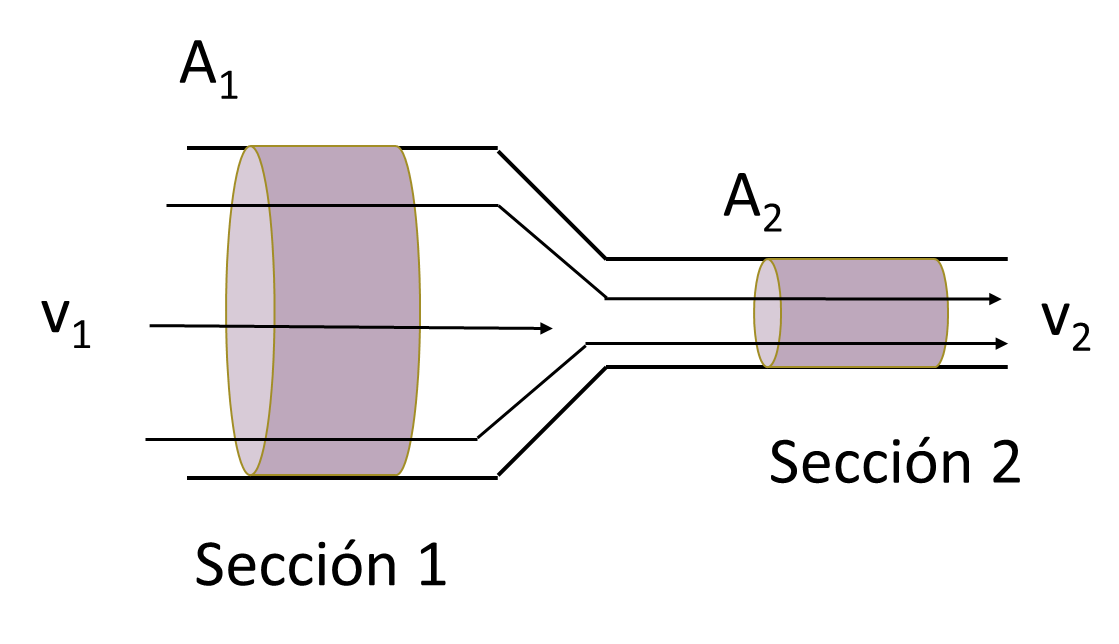
\includegraphics[scale=0.8]{Imagenes/Ejercicio_Bernoulli_01.png}
\end{figure}
\end{frame}
\begin{frame}
\frametitle{Ejercicio - Ec. de Bernoulli}
La velocidad en la sección 1 es de \SI[per-mode=symbol]{4}{\meter\per\second} a una presión de \SI{4d5}{\pascal}. Por la tubería circula agua.
\\
\bigskip
\pause
¿Cuál es la velocidad y presión en la sección 2?
\end{frame}
\begin{frame}
\frametitle{Resolviendo el ejercicio}
\vspace*{-1cm}
\begin{minipage}[t]{0.4\linewidth}
\textocolor{red}{Datos:}
\begin{align*}
v_{2} &= ? \\[0.25em]
P_{2} &= ? \\[0.25em]
A_{1} &= \SI{0.02}{\square\meter} \\[0.25em]
A_{2} &= \SI{0.01}{\square\meter} \\[0.25em]
\end{align*}
\end{minipage}
\begin{minipage}[t]{0.4\linewidth}
\begin{align*}
\rho &= \SI{1000}{\kilo\gram\per\cubic\meter} \\[0.25em]
v_{1} &= \SI{4}{\meter\per\second} \\[0.25em]
P_{1} &= \SI{4d5}{\pascal}
\end{align*}
\end{minipage}
\end{frame}
\begin{frame}
\frametitle{Resolviendo el ejercicio}
\textocolor{red}{Datos:} Ecuación de continuidad:
\pause
\begin{eqnarray*}
\begin{aligned}
v_{1} \, A_{1} = v_{2} \, A_{2} \pause \hspace*{0.2cm} \Rightarrow \hspace*{0.2cm} v_{2} = \dfrac{v_{1} \, A_{1}}{a_{2}}
\end{aligned}
\end{eqnarray*}
\pause
Ecuación de Bernoulli:
\pause
\begin{align*}
P_{1} + \rho \, g \, h_{1} + \dfrac{1}{2} \rho \, v_{1}^{2} = P_{2} + \rho \, g \, h_{2} + \dfrac{1}{2} \rho \, v_{2}^{2}
\end{align*}
\end{frame}
\begin{frame}
\frametitle{Resolviendo el ejercicio}
\textocolor{red}{Sustitución:} Ecuación de continuidad:
\pause
\begin{eqnarray*}
\begin{aligned}
v_{2} &= \dfrac{\left( \displaystyle \SI[per-mode=fraction]{4}{\meter\per\second}\right) \left( \SI{0.02}{\square\meter}\right)}{\SI{0.01}{\square\meter}} = \\[0.5em] \pause
v_{2} &= \dfrac{ \displaystyle \SI{0.08}{\square\meter} \si[per-mode=fraction]{\meter\per\second}}{\SI{0.01}{\square\meter}} =  \\[0.5em] \pause
v_{2} &= \SI[per-mode=fraction]{8}{\meter\per\second}
\end{aligned}
\end{eqnarray*}
\end{frame}
\begin{frame}
\frametitle{Resolviendo el ejercicio}
\textocolor{red}{Sustitución:} Ecuación de Bernoulli, \pause En este ejercicio consideramos que las alturas $h_{1}$ y $h_{2}$, son iguales, es decir $h_{1} = h_{2} = h$.
\pause
\begin{eqnarray*}
\begin{aligned}
&P_{1} + \rho \, g \, h + \dfrac{1}{2} \rho \, v_{1}^{2} = P_{2} + \rho \, g \, h + \dfrac{1}{2} \rho \, v_{2}^{2} \\[0.5em] \pause
&\Rightarrow \hspace{0.4cm} P_{1} + \rho \, g \, (h - h) + \dfrac{1}{2} \rho \, v_{1}^{2} = P_{2} + \dfrac{1}{2} \rho \, v_{2}^{2}
\end{aligned}
\end{eqnarray*}
\end{frame}
\begin{frame}
\frametitle{Resolviendo el ejercicio}
\vspace*{-1cm}
\begin{eqnarray*}
\begin{aligned}
&P_{1} + \dfrac{1}{2} \rho \, v_{1}^{2} = P_{2} + \dfrac{1}{2} \rho \, v_{2}^{2} \\[0.5em] \pause
&P_{2} - P_{1} = \dfrac{1}{2} \rho \, v_{1}^{2} - \dfrac{1}{2} \rho \, v_{2}^{2} \\[0.5em] \pause
&P_{2} - P_{1} = \dfrac{1}{2} \rho \, \left( v_{1}^{2} - v_{2}^{2} \right) \\[0.5em] \pause
&P_{2} = \dfrac{1}{2} \rho \, \left( v_{1}^{2} - v_{2}^{2} \right) + P_{1}
\end{aligned}
\end{eqnarray*}
\end{frame}
\begin{frame}
\frametitle{Resolviendo el ejercicio}
\vspace*{-1cm}
\begin{eqnarray*}
\begin{aligned}
P_{2} &= \dfrac{1}{2} \rho \, \left( v_{1}^{2} - v_{2}^{2} \right) + P_{1} = \\[0.5em] \pause
P_{2} &= \dfrac{1}{2} \left( \SI[per-mode=fraction]{d3}{\kilo\gram\per\cubic\meter} \right) \, \left[ \left( \SI[per-mode=fraction]{4}{\meter\per\second} \right)^{2} - \left( \SI[per-mode=fraction]{8}{\meter\per\second} \right)^{2} \right] + \SI{4d5}{\pascal} =  \\[0.5em] \pause
P_{2} &= - \SI{2.4d4}{\pascal} + \SI{4d5}{\pascal} =  \\[0.5em] \pause
P_{2} &= \SI{3.76d5}{\pascal}
\end{aligned}
\end{eqnarray*}
\end{frame}

\section{Tipos de flujo}
\frame{\tableofcontents[currentsection, hideothersubsections]}
\subsection{Fluidos en movimiento}

\begin{frame}
\frametitle{Fluidos en movimiento}
El \textocolor{byzantine}{flujo laminar} y el \textocolor{ao}{flujo turbulento} son dos regímenes distintos de movimiento de un fluido, \pause se utilizan en la mecánica de fluidos para describir cómo se comporta un fluido en movimiento.
\end{frame}

\subsection{Flujo laminar} 

\begin{frame}
\frametitle{Definición}
En el flujo laminar, las partículas del fluido \textocolor{burgundy}{se mueven en capas o láminas paralelas} sin cruzarse significativamente.
\end{frame}
\begin{frame}
\frametitle{Características} 
Las partículas se mueven de manera ordenada y predecible.
\\
\bigskip
\pause
No hay remolinos ni turbulencias notables. \pause La velocidad del fluido en cada capa es constante y su dirección no cambia abruptamente.
\end{frame}
\begin{frame}
\frametitle{Condición de Transición}
El flujo puede volverse laminar a velocidades bajas y viscosidades altas.
\end{frame}
\begin{frame}
\frametitle{Ejemplo}
El flujo de aceite a través de una tubería de pequeño diámetro a velocidades moderadas puede ser laminar.
\end{frame}
\begin{frame}
\frametitle{Ejemplo flujo sanguíneo}
En arterias más pequeñas y capilares, donde el flujo es más lento y las paredes de los vasos son más suaves, es más probable que se dé un flujo laminar.
\end{frame}
\begin{frame}
\frametitle{Ejemplo flujo sanguíneo}
El flujo es ordenado, capa tras capa, y no hay interrupciones significativas en la dirección del flujo.
\end{frame}
\begin{frame}
\frametitle{Ejemplo flujo sanguíneo}
El flujo laminar permite un transporte eficiente de nutrientes y gases a través de las paredes de los vasos sanguíneos hacia los tejidos.
\end{frame}

\subsection{Flujo turbulento}

\begin{frame}
\frametitle{Definición}
En el flujo turbulento, las partículas del fluido \textocolor{cardinal}{se mezclan de manera caótica} y se generan remolinos y fluctuaciones en la velocidad y la presión.
\end{frame}
\begin{frame}
\frametitle{Características}
Existen vórtices y corrientes cruzadas en el fluido.
\\
\bigskip
\pause
La velocidad y la dirección del fluido son variables y cambian continuamente. \pause Se producen pérdidas de energía debido a la fricción interna.
\end{frame}
\begin{frame}
\frametitle{Condición de Transición}
El flujo se vuelve turbulento a velocidades más altas y viscosidades más bajas.
\end{frame}
\begin{frame}
\frametitle{Ejemplo}
El agua fluyendo por una cascada o un río con obstáculos puede exhibir flujo turbulento.
\end{frame}
\begin{frame}
\frametitle{Ejemplo flujo sanguíneo}
En arterias más grandes y en áreas donde la velocidad del flujo es alta, como en las bifurcaciones y curvas, puede ocurrir el flujo turbulento.
\end{frame}
\begin{frame}
\frametitle{Ejemplo flujo sanguíneo}
El flujo es caótico, con remolinos y fluctuaciones en la velocidad y la presión.
\end{frame}
\begin{frame}
\frametitle{Ejemplo flujo sanguíneo}
La presencia de \textocolor{bole}{placas ateroscleróticas} puede causar turbulencias y cambios en el flujo sanguíneo.
\end{frame}

\subsection{Número de Reynolds}

\begin{frame}
\frametitle{Definición}
El \textocolor{red}{número de Reynolds (Re)} es un parámetro adimensional utilizado para predecir cuándo un flujo transita de laminar a turbulento.
\end{frame}
\begin{frame}
\frametitle{Definición}
Se define como la relación entre las fuerzas inerciales y las fuerzas viscosas del fluido.
\end{frame}
\begin{frame}
\frametitle{Rangos para Re}
Si $Re < 2300$, generalmente indica \textocolor{darkscarlet}{flujo laminar}, \pause mientras que $Re > 4000$ indica \textocolor{debianred}{flujo turbulento}.
\end{frame}
\begin{frame}
\frametitle{Relevancia de Re}
La transición entre flujo laminar y turbulento es importante en muchos campos de la ciencia e ingeniería.
\end{frame}
\begin{frame}
\frametitle{Relevancia de Re}
Ya que afecta la eficiencia de:
\setbeamercolor{item projected}{bg=coquelicot,fg=black}
\setbeamertemplate{enumerate items}{%
\usebeamercolor[bg]{item projected}%
\raisebox{1.5pt}{\colorbox{bg}{\color{fg}\footnotesize\insertenumlabel}}%
}
\begin{enumerate}[<+->]
\item Transferencia de calor.
\item La resistencia al flujo.
\item Así como otros aspectos del comportamiento del fluido en sistemas como tuberías, conductos y canales.
\end{enumerate}
\end{frame}


\end{document}